\documentclass[conference]{IEEEtran}
%DIF LATEXDIFF DIFFERENCE FILE
%DIF DEL /tmp/main_submitted.tex   Sat Oct 10 01:10:02 2026
%DIF ADD main.tex                  Sat Oct 10 01:07:19 2026
\IEEEoverridecommandlockouts
\usepackage{cite}
\usepackage{amsmath,amssymb,amsfonts}
\usepackage{graphicx}
\usepackage{textcomp}
\usepackage{booktabs}
\usepackage{xcolor}
\usepackage{url}

%DIF 11-19c11-12
%DIF < \def\BibTeX{{\rm B\kern-.05em{\sc i\kern-.025em b}\kern-.08em
%DIF <     T\kern-.1667em\lower.7ex\hbox{E}\kern-.125emX}}
%DIF < 
%DIF < % Compact spacing (page-budget only, IEEEtran-compatible): default float/
%DIF < % caption skips are generous for a conference two-column layout; tightened
%DIF < % here so a content-heavy 5-page paper fits without shrinking fonts/margins.
%DIF < \setlength{\textfloatsep}{3pt plus 2pt minus 2pt}
%DIF < \setlength{\floatsep}{2pt plus 2pt minus 2pt}
%DIF < \setlength{\intextsep}{3pt plus 2pt minus 2pt}
%DIF -------
\setlength{\textfloatsep}{4pt plus 2pt minus 2pt}
 %DIF > 
\setlength{\floatsep}{3pt plus 2pt minus 2pt}
 %DIF > 
%DIF -------
\setlength{\abovecaptionskip}{2pt}
\setlength{\belowcaptionskip}{1pt}
%DIF 22-29c15
%DIF < \renewcommand{\arraystretch}{0.85}
%DIF < % Bibliography-only: IEEEtran's default per-entry list spacing is more
%DIF < % generous than a 21-entry, footnotesize reference list needs; tightened
%DIF < % here rather than shrinking the two enlarged figures back down again
%DIF < % (user preference, this round). \bibsep itself is a natbib length, not
%DIF < % defined by plain IEEEtran, so the standard robust trick is used instead:
%DIF < % wrap \thebibliography (always a list environment, whatever the class)
%DIF < % and tighten \itemsep/\parskip inside it directly.
%DIF -------
\renewcommand{\arraystretch}{0.9}
 %DIF > 
%DIF -------
\let\IEEEoldthebibliography\thebibliography
\renewcommand{\thebibliography}[1]{%
  \IEEEoldthebibliography{#1}%
  \setlength{\itemsep}{0pt plus 0.3ex}%
  \setlength{\parskip}{0pt}%
}
%DIF 36-38d22
%DIF < % Allow a little extra justification slack (standard, invisible at this
%DIF < % magnitude) so dense technical text and long bibliography URLs don't throw
%DIF < % sub-pixel overfull/underfull hbox warnings.
%DIF -------
\emergencystretch=2em
%DIF < \hfuzz=20pt
%DIF -------

 %DIF > 
%DIF < \vbadness=10000
%DIF PREAMBLE EXTENSION ADDED BY LATEXDIFF
%DIF UNDERLINE PREAMBLE %DIF PREAMBLE
\RequirePackage[normalem]{ulem} %DIF PREAMBLE
\RequirePackage{color}\definecolor{RED}{rgb}{1,0,0}\definecolor{BLUE}{rgb}{0,0,1} %DIF PREAMBLE
\providecommand{\DIFadd}[1]{{\protect\color{blue}\uwave{#1}}} %DIF PREAMBLE
\providecommand{\DIFdel}[1]{{\protect\color{red}\sout{#1}}} %DIF PREAMBLE
%DIF SAFE PREAMBLE %DIF PREAMBLE
\providecommand{\DIFaddbegin}{} %DIF PREAMBLE
\providecommand{\DIFaddend}{} %DIF PREAMBLE
\providecommand{\DIFdelbegin}{} %DIF PREAMBLE
\providecommand{\DIFdelend}{} %DIF PREAMBLE
\providecommand{\DIFmodbegin}{} %DIF PREAMBLE
\providecommand{\DIFmodend}{} %DIF PREAMBLE
%DIF FLOATSAFE PREAMBLE %DIF PREAMBLE
\providecommand{\DIFaddFL}[1]{\DIFadd{#1}} %DIF PREAMBLE
\providecommand{\DIFdelFL}[1]{\DIFdel{#1}} %DIF PREAMBLE
\providecommand{\DIFaddbeginFL}{} %DIF PREAMBLE
\providecommand{\DIFaddendFL}{} %DIF PREAMBLE
\providecommand{\DIFdelbeginFL}{} %DIF PREAMBLE
\providecommand{\DIFdelendFL}{} %DIF PREAMBLE
\providecommand{\DIFscaledelfig}{0.5}
%DIF HIGHLIGHTGRAPHICS PREAMBLE %DIF PREAMBLE
\RequirePackage{settobox} %DIF PREAMBLE
\RequirePackage{letltxmacro} %DIF PREAMBLE
\newsavebox{\DIFdelgraphicsbox} %DIF PREAMBLE
\newlength{\DIFdelgraphicswidth} %DIF PREAMBLE
\newlength{\DIFdelgraphicsheight} %DIF PREAMBLE
% store original definition of \includegraphics %DIF PREAMBLE
\LetLtxMacro{\DIFOincludegraphics}{\includegraphics} %DIF PREAMBLE
\providecommand{\DIFaddincludegraphics}[2][]{{\color{blue}\fbox{\DIFOincludegraphics[#1]{#2}}}} %DIF PREAMBLE
\providecommand{\DIFdelincludegraphics}[2][]{% %DIF PREAMBLE
\sbox{\DIFdelgraphicsbox}{\DIFOincludegraphics[#1]{#2}}% %DIF PREAMBLE
\settoboxwidth{\DIFdelgraphicswidth}{\DIFdelgraphicsbox} %DIF PREAMBLE
\settoboxtotalheight{\DIFdelgraphicsheight}{\DIFdelgraphicsbox} %DIF PREAMBLE
\scalebox{\DIFscaledelfig}{% %DIF PREAMBLE
\parbox[b]{\DIFdelgraphicswidth}{\usebox{\DIFdelgraphicsbox}\\[-\baselineskip] \rule{\DIFdelgraphicswidth}{0em}}\llap{\resizebox{\DIFdelgraphicswidth}{\DIFdelgraphicsheight}{% %DIF PREAMBLE
\setlength{\unitlength}{\DIFdelgraphicswidth}% %DIF PREAMBLE
\begin{picture}(1,1)% %DIF PREAMBLE
\thicklines\linethickness{2pt} %DIF PREAMBLE
{\color[rgb]{1,0,0}\put(0,0){\framebox(1,1){}}}% %DIF PREAMBLE
{\color[rgb]{1,0,0}\put(0,0){\line( 1,1){1}}}% %DIF PREAMBLE
{\color[rgb]{1,0,0}\put(0,1){\line(1,-1){1}}}% %DIF PREAMBLE
\end{picture}% %DIF PREAMBLE
}\hspace*{3pt}}} %DIF PREAMBLE
} %DIF PREAMBLE
\LetLtxMacro{\DIFOaddbegin}{\DIFaddbegin} %DIF PREAMBLE
\LetLtxMacro{\DIFOaddend}{\DIFaddend} %DIF PREAMBLE
\LetLtxMacro{\DIFOdelbegin}{\DIFdelbegin} %DIF PREAMBLE
\LetLtxMacro{\DIFOdelend}{\DIFdelend} %DIF PREAMBLE
\DeclareRobustCommand{\DIFaddbegin}{\DIFOaddbegin \let\includegraphics\DIFaddincludegraphics} %DIF PREAMBLE
\DeclareRobustCommand{\DIFaddend}{\DIFOaddend \let\includegraphics\DIFOincludegraphics} %DIF PREAMBLE
\DeclareRobustCommand{\DIFdelbegin}{\DIFOdelbegin \let\includegraphics\DIFdelincludegraphics} %DIF PREAMBLE
\DeclareRobustCommand{\DIFdelend}{\DIFOaddend \let\includegraphics\DIFOincludegraphics} %DIF PREAMBLE
\LetLtxMacro{\DIFOaddbeginFL}{\DIFaddbeginFL} %DIF PREAMBLE
\LetLtxMacro{\DIFOaddendFL}{\DIFaddendFL} %DIF PREAMBLE
\LetLtxMacro{\DIFOdelbeginFL}{\DIFdelbeginFL} %DIF PREAMBLE
\LetLtxMacro{\DIFOdelendFL}{\DIFdelendFL} %DIF PREAMBLE
\DeclareRobustCommand{\DIFaddbeginFL}{\DIFOaddbeginFL \let\includegraphics\DIFaddincludegraphics} %DIF PREAMBLE
\DeclareRobustCommand{\DIFaddendFL}{\DIFOaddendFL \let\includegraphics\DIFOincludegraphics} %DIF PREAMBLE
\DeclareRobustCommand{\DIFdelbeginFL}{\DIFOdelbeginFL \let\includegraphics\DIFdelincludegraphics} %DIF PREAMBLE
\DeclareRobustCommand{\DIFdelendFL}{\DIFOaddendFL \let\includegraphics\DIFOincludegraphics} %DIF PREAMBLE
%DIF AMSMATHULEM PREAMBLE %DIF PREAMBLE
\makeatletter %DIF PREAMBLE
\let\sout@orig\sout %DIF PREAMBLE
\renewcommand{\sout}[1]{\ifmmode\text{\sout@orig{\ensuremath{#1}}}\else\sout@orig{#1}\fi} %DIF PREAMBLE
\makeatother %DIF PREAMBLE
%DIF COLORLISTINGS PREAMBLE %DIF PREAMBLE
\RequirePackage{listings} %DIF PREAMBLE
\RequirePackage{color} %DIF PREAMBLE
\lstdefinelanguage{DIFcode}{ %DIF PREAMBLE
%DIF DIFCODE_UNDERLINE %DIF PREAMBLE
  moredelim=[il][\color{red}\sout]{\%DIF\ <\ }, %DIF PREAMBLE
  moredelim=[il][\color{blue}\uwave]{\%DIF\ >\ } %DIF PREAMBLE
} %DIF PREAMBLE
\lstdefinestyle{DIFverbatimstyle}{ %DIF PREAMBLE
	language=DIFcode, %DIF PREAMBLE
	basicstyle=\ttfamily, %DIF PREAMBLE
	columns=fullflexible, %DIF PREAMBLE
	keepspaces=true %DIF PREAMBLE
} %DIF PREAMBLE
\lstnewenvironment{DIFverbatim}[1][]{\lstset{style=DIFverbatimstyle}}{} %DIF PREAMBLE
\lstnewenvironment{DIFverbatim*}[1][]{\lstset{style=DIFverbatimstyle,showspaces=true}}{} %DIF PREAMBLE
\lstset{extendedchars=\true,inputencoding=utf8}

%DIF END PREAMBLE EXTENSION ADDED BY LATEXDIFF

\begin{document}

\title{Physics-Informed Graph Neural Networks with Uncertainty Quantification \DIFdelbegin \DIFdel{: A Pre-Registered Evaluation Protocol }\DIFdelend for \DIFaddbegin \DIFadd{Conservative, Registry-Compatible }\DIFaddend Blue Carbon \DIFdelbegin \DIFdel{Credit Pricing}\DIFdelend \DIFaddbegin \DIFadd{Crediting}\DIFaddend }

\author{
\IEEEauthorblockN{Nahla Nabil Skaik}
\DIFdelbegin %DIFDELCMD < \IEEEauthorblockA{Arab Open University, Bahrain\\
%DIFDELCMD < nahla.nabil.52@gmail.com}
%DIFDELCMD < %%%
\DIFdelend \DIFaddbegin \IEEEauthorblockA{Faculty of Computer Studies\\
Arab Open University\\
Kingdom of Bahrain\\
Email: nahla.nabil.52@gmail.com}
\DIFaddend }

\maketitle

\begin{abstract}
\DIFdelbegin \DIFdel{Flat, rule-based }\DIFdelend \DIFaddbegin \DIFadd{Mangrove carbon credits are discounted by a }\DIFaddend non-permanence \DIFdelbegin \DIFdel{buffers discount every credit in a
voluntary carbon market identically, regardless of }\DIFdelend \DIFaddbegin \DIFadd{buffer that ignores how uncertain }\DIFaddend the underlying carbon-stock estimate \DIFdelbegin \DIFdel{'s confidence.
We test whether }\DIFdelend \DIFaddbegin \DIFadd{is.
In this study, }\DIFaddend a physics-informed graph neural network (GNN) \DIFdelbegin \DIFdel{with conformalized quantile regression (CQR)
can supply a per-site confidence signal that complements, rather than
replaces, this buffer, on a 10,124-node spatial graph of the Ten
Thousand Islands mangrove fringe, southwest Florida
(Sentinel-2, Global Mangrove Watch, field-calibrated }\DIFdelend \DIFaddbegin \DIFadd{and gradient-boosted trees are combined to map }\DIFaddend soil organic carbon \DIFdelbegin \DIFdel{). Model selection (physics-loss weight,feature set,calibration
method)was pre-registered on validation data and confirmed once on a held-out test block.
A five-seed check found }\DIFdelend \DIFaddbegin \DIFadd{over two southwest Florida mangrove regions (10,124 and 22,326 nodes of 150\,m), and conformal prediction turns each estimate into a calibrated 90\% interval that feeds the uncertainty deduction of the Verra VM0033 methodology.
Spatial cross-validation selected an ensemble of }\DIFaddend the physics-informed \DIFdelbegin \DIFdel{loss's
point-accuracy advantage over a no-physics GNN did not replicate: on
test, the no-physics GNN has the best $R^2$ of three models ($-0.383$
vs.\ $-0.430$ physics-informed and $-0.450$ linear). Its predictions do
correlate most strongly with the imposed physical prior on held-out
nodes($0.755$ vs.\ $0.682$/$0.686$), evidence the constraint transfers
under spatial shift, not independent physical validation, }\DIFdelend \DIFaddbegin \DIFadd{GNN and XGBoost (cross-validated $R^2=0.47$ and 0.55), which reached test $R^2=0.28$ }\DIFaddend and \DIFdelbegin \DIFdel{a real but
much smaller margin than an earlier single-seed pilot suggested. Global
CQR calibration reached 91.1\% /96.4\% coverage at 90\%/95\%nominal; a spatially localized (Mondrian) variant undercovered more on test
(83.4\% , 92.4\%), a genuine negative result consistent with
spatial-conformal theory's local-density requirement.
A pricing
proof-of-concept built on the better-calibrated global intervals maps
interval width to a multiplier ranging $0.50$--$1.50$ across five test
nodes, against Plan Vivo's fixed $0.800$ flat-buffer multiplier.
Point-prediction accuracy remains weak throughout; the contribution is
the pre-registered protocol itself, which caught both a single-run
estimate and a calibration refinement overstating their reliability, not
validated point accuracy or a validated pricing model}\DIFdelend \DIFaddbegin \DIFadd{0.60 against 0.20 and 0.59 for XGBoost alone.
Conformal intervals covered 91.5\% and 89.1\% of test nodes, with interval width tracking absolute error (Spearman $\rho=0.54$ in the first region).
The registry rule withheld a median 12.7\% and 2.1\% of credits per node, an amount comparable to the 11.0\% median buffer that seven issuing blue carbon projects actually hold.
Aggregating node uncertainty as the methodology prescribes, assuming independent errors, covered only 18\% and 33\% of realized project-level errors on validation data, while a correlation-aware aggregation covered at least 91\%.
Against 87 field soil cores, the ensemble's site-level median error was 10.1\%, below a constant regional mean (15.0\%) and two published carbon maps (14.1\% and 15.1\%)}\DIFaddend .
\DIFaddbegin \DIFadd{These results support crediting rules that keep estimation uncertainty separate from non-permanence risk and that aggregate it under spatially correlated errors.
}\DIFaddend \end{abstract}

\begin{IEEEkeywords}
blue carbon, graph neural \DIFdelbegin \DIFdel{network, physics-informed learning, }\DIFdelend \DIFaddbegin \DIFadd{networks, }\DIFaddend conformal prediction, \DIFdelbegin \DIFdel{uncertainty quantification, carbon credit pricing
}\DIFdelend \DIFaddbegin \DIFadd{carbon credits, uncertainty quantification
}\DIFaddend \end{IEEEkeywords}

\section{Introduction}

Voluntary carbon markets discount mangrove credits for non-permanence risk (carbon later released \DIFdelbegin \DIFdel{via }\DIFdelend \DIFaddbegin \DIFadd{through }\DIFaddend erosion, sea-level rise \DIFdelbegin \DIFdel{, }\DIFdelend or disturbance) \DIFdelbegin \DIFdel{using a buffer pool: a fixed percentage }\DIFdelend \DIFaddbegin \DIFadd{by withholding a fixed share }\DIFaddend of issued credits \DIFdelbegin \DIFdel{withheld from
sale, unconditioned on how confident the underlying carbon-stock estimate
is}\DIFdelend \DIFaddbegin \DIFadd{in a buffer pool \mbox{%DIFAUXCMD
\cite{verra_vm0033,planvivo_buffer}}\hskip0pt%DIFAUXCMD
.
That share does not depend on how well the carbon stock itself was estimated}\DIFaddend .
Verra's VM0033 \DIFdelbegin \DIFdel{and Plan Vivo V5.0 both apply this uniformly,
regardless of sub-project granularity
\mbox{%DIFAUXCMD
\cite{verra_vm0033,planvivo_buffer}}\hskip0pt%DIFAUXCMD
, and existing }\DIFdelend \DIFaddbegin \DIFadd{methodology does contain a separate uncertainty deduction: credits are reduced when the 90\% confidence interval exceeds 20\% of the estimate \mbox{%DIFAUXCMD
\cite{verra_vm0033}}\hskip0pt%DIFAUXCMD
.
In practice, the }\DIFaddend carbon-stock \DIFdelbegin \DIFdel{models for this ecosystem and region report only point estimates , }\DIFdelend \DIFaddbegin \DIFadd{maps available for mangroves report point estimates }\DIFaddend with no calibrated \DIFdelbegin \DIFdel{per-prediction confidence a pricing rule could condition on
\mbox{%DIFAUXCMD
\cite{radabaugh2023bluecarbon,sanderman2023soc,simard2019mangrove}}\hskip0pt%DIFAUXCMD
.
Conformal prediction supplies valid, distribution-free uncertainty for
earth-observation and spatial regression
\mbox{%DIFAUXCMD
\cite{eo_conformal2024,lou2024geoconformal,gonzalezabad2023ensembles}}\hskip0pt%DIFAUXCMD
,
but no existing work pairs that calibrated uncertainty with a physics-informed spatial predictor, couples it to a buffer-pool pricing
mechanism, or tests whether a calibration strategy (global versus
spatially localized) holds under one region's calibration-density
constraints, the narrower gap this paper addresses (Section~II surveys
each literature in full).
This paper combines a }\DIFdelend \DIFaddbegin \DIFadd{per-site interval \mbox{%DIFAUXCMD
\cite{sanderman2023soc,radabaugh2023bluecarbon}}\hskip0pt%DIFAUXCMD
, and the methodology combines plot uncertainties under an independence assumption that spatial models rarely satisfy.

}

\DIFadd{This paper asks whether calibrated, per-site uncertainty from a spatial model can supply that deduction in a way a registry could audit.
A }\DIFaddend physics-informed graph neural network \DIFdelbegin \DIFdel{\mbox{%DIFAUXCMD
\cite{raissi2019pinn,sanchezgonzalez2020gns}}\hskip0pt%DIFAUXCMD
, previously
applied to mass-conserving flood forecasting
\mbox{%DIFAUXCMD
\cite{taghizadeh2025floodpignn,dualfloodgnn2025} }\hskip0pt%DIFAUXCMD
but not, to our
knowledge, blue carbon, with }\DIFdelend \DIFaddbegin \DIFadd{\mbox{%DIFAUXCMD
\cite{raissi2019pinn,hamilton2017graphsage} }\hskip0pt%DIFAUXCMD
encodes neighborhood structure and a tidal-inundation prior; tree ensembles \mbox{%DIFAUXCMD
\cite{breiman2001rf,chen2016xgboost} }\hskip0pt%DIFAUXCMD
supply strong tabular baselines; and conformalized quantile regression \mbox{%DIFAUXCMD
\cite{romano2019cqr} }\hskip0pt%DIFAUXCMD
gives }\DIFaddend distribution-free \DIFdelbegin \DIFdel{uncertainty calibration
to test whether estimation confidence can complement, not replace, a flat }\DIFdelend \DIFaddbegin \DIFadd{intervals.
This study differs from previous research in four ways: (1) the interval of every node is converted into the VM0033 deduction, kept separate from the }\DIFaddend non-permanence \DIFdelbegin \DIFdel{discount.
}%DIFDELCMD < 

%DIFDELCMD < %%%
\DIFdel{The scope is deliberately narrow: one pilot region, one physics constraint
(a steady-state mass-balance proxy, not a full temporal flux equation) ,
and one primary UQ method (CQR; deep ensembles and MC dropout are left
for future work) . Every model-selection decision, physics-loss weight,
feature set, calibration method, was pre-registered on a validation
split and confirmed once on a spatially distinct test block never used
for any prior decision; we treat this two-stage protocol itself as a
methodological contribution (Section~III-C) , since a naive single-run
estimate and a theoretically-motivated calibration refinement each turned
out to mislead here (Section~V) . What survives that scrutiny is smaller
and more tightly bounded than either initial result suggested: a real
but modest prior-generalization advantage for the physics-informed model, and evidence that localized (Mondrian) conformal calibration, plausible
in theory and competitive on validation-internal evidence, underperforms
the simpler global variant on this AOI's test data }\DIFdelend \DIFaddbegin \DIFadd{buffer and compared with the buffers held by issuing projects \mbox{%DIFAUXCMD
\cite{vrod2026}}\hskip0pt%DIFAUXCMD
; (2) the methodology's own aggregation rule is tested empirically and shown to understate project-level uncertainty when model errors are spatially correlated; (3) predictions and published maps are checked against 87 independent field soil cores \mbox{%DIFAUXCMD
\cite{ccn2023library}}\hskip0pt%DIFAUXCMD
; and (4) the analysis covers two regions, two image dates and leakage-free spatial splits, with every model choice fixed on validation data under rules committed before the experiments were run.

}

\DIFadd{The scope is deliberately applied: the paper does not propose a new network architecture.
The contribution is a crediting pipeline whose uncertainty is calibrated, auditable and conservative, together with evidence on where that uncertainty is and is not informative}\DIFaddend .

\DIFdelbegin \DIFdel{The contribution is
this pre-registered evaluation and its honest limits, not a validated
point-prediction accuracy claim or a validated pricing model.
}\DIFdelend 

\section{Related Work}

\DIFdelbegin %DIFDELCMD < \textbf{Physics-informed GNNs.} %%%
\DIFdelend \DIFaddbegin \textbf{Physics-informed and graph learning.} \DIFaddend Physics-guided \DIFdelbegin \DIFdel{ML integrates
scientific structure into learned }\DIFdelend \DIFaddbegin \DIFadd{learning adds scientific structure to data-driven }\DIFaddend models \cite{willard2022piml}; \DIFdelbegin \DIFdel{PINNs add
a PDE-residual loss \mbox{%DIFAUXCMD
\cite{raissi2019pinn}}\hskip0pt%DIFAUXCMD
, Graph Network Simulators encode
physics via local, permutation-invariant message passing
\mbox{%DIFAUXCMD
\cite{sanchezgonzalez2020gns}}\hskip0pt%DIFAUXCMD
. The closest prior art, flood forecasting \mbox{%DIFAUXCMD
\cite{taghizadeh2025floodpignn, dualfloodgnn2025}}\hskip0pt%DIFAUXCMD
, is entirely
hydrological and does not target mangrove carbon or couple prediction to
a priced instrument via UQ.
}\DIFdelend \DIFaddbegin \DIFadd{physics-informed networks penalize violations of governing equations \mbox{%DIFAUXCMD
\cite{raissi2019pinn}}\hskip0pt%DIFAUXCMD
, and graph formulations have carried such constraints into flood forecasting \mbox{%DIFAUXCMD
\cite{taghizadeh2025floodpignn}}\hskip0pt%DIFAUXCMD
.
GraphSAGE \mbox{%DIFAUXCMD
\cite{hamilton2017graphsage} }\hskip0pt%DIFAUXCMD
learns from node neighborhoods inductively, which suits spatial grids split into separate regions.

}\DIFaddend 

\DIFdelbegin %DIFDELCMD < \textbf{Mangrove carbon stock estimation.} %%%
\DIFdel{The dominant approach is
per-pixel tabular regression (random forest, XGBoost) }\DIFdelend \DIFaddbegin \textbf{Mangrove carbon mapping.} \DIFadd{Most mangrove carbon studies regress field or map values }\DIFaddend on spectral indices \DIFdelbegin \DIFdel{. Simard et al.'s global mangrove biomass product
\mbox{%DIFAUXCMD
\cite{simard2019mangrove} }\hskip0pt%DIFAUXCMD
was inaccessible here (NASA Earthdata
login required). }\DIFdelend \DIFaddbegin \DIFadd{with random forests or boosted trees \mbox{%DIFAUXCMD
\cite{roy2024mangroveasiapacific}}\hskip0pt%DIFAUXCMD
.
Global soil carbon products are themselves machine-learning outputs \mbox{%DIFAUXCMD
\cite{sanderman2018map,sanderman2023soc}}\hskip0pt%DIFAUXCMD
, and regional maps such as }\DIFaddend Radabaugh et al.\ \DIFdelbegin \DIFdel{built a field-plot-calibrated, 30\,m
carbon-stock model for the southwest Florida coast, one sub-region
matching our pilot AOI \mbox{%DIFAUXCMD
\cite{radabaugh2023bluecarbon} }\hskip0pt%DIFAUXCMD
}\DIFdelend \DIFaddbegin \DIFadd{\mbox{%DIFAUXCMD
\cite{radabaugh2023bluecarbon} }\hskip0pt%DIFAUXCMD
are calibrated on local field cores.
Geomorphic setting and tidal regime control mangrove soil carbon \mbox{%DIFAUXCMD
\cite{rovai2018controls,krauss2014sealevel}}\hskip0pt%DIFAUXCMD
, and soil carbon maps can disagree substantially at fine scales \mbox{%DIFAUXCMD
\cite{holmquist2018tidal}}\hskip0pt%DIFAUXCMD
.
Random cross-validation overstates accuracy on such data; spatial blocking is required \mbox{%DIFAUXCMD
\cite{roberts2017cv,ploton2020spatial}}\hskip0pt%DIFAUXCMD
}\DIFaddend .

\DIFdelbegin \DIFdel{Sanderman et
al.\ produced the global, field-calibrated 30\,m SOC product
\mbox{%DIFAUXCMD
\cite{sanderman2023soc} }\hskip0pt%DIFAUXCMD
we train against. A 105-study review confirms
belowground-carbon and valuation research remain under-studied versus
aboveground biomass \mbox{%DIFAUXCMD
\cite{roy2024mangroveasiapacific}}\hskip0pt%DIFAUXCMD
.
None uses a graph
representation or a physical constraint, or reports a calibrated
uncertainty interval (the gap this paper addresses).
}\DIFdelend 

\textbf{Uncertainty quantification.} \DIFdelbegin \DIFdel{MC dropout \mbox{%DIFAUXCMD
\cite{gal2016dropout} }\hskip0pt%DIFAUXCMD
is
cheap but poorly calibrated under shift; deep ensembles
\mbox{%DIFAUXCMD
\cite{lakshminarayanan2017ensembles} }\hskip0pt%DIFAUXCMD
calibrate better but need multiple
full models, as in climate-downscaling \mbox{%DIFAUXCMD
\cite{gonzalezabad2023ensembles}}\hskip0pt%DIFAUXCMD
.
CQR \mbox{%DIFAUXCMD
\cite{romano2019cqr} }\hskip0pt%DIFAUXCMD
turns a point predictor into calibrated intervals with a coverage guarantee that holds without distributional
assumptions, so long as calibration and test data are exchangeable, validated for earth observation \mbox{%DIFAUXCMD
\cite{eo_conformal2024}}\hskip0pt%DIFAUXCMD
; that guarantee
is conditional on exchangeability spatial autocorrelation can violate. GeoConformal Prediction
\mbox{%DIFAUXCMD
\cite{lou2024geoconformal} }\hskip0pt%DIFAUXCMD
addresses this with a spatially localized
framework, motivating the Mondrian variant we test (Section~III-F) }\DIFdelend \DIFaddbegin \DIFadd{Split conformal prediction gives finite-sample coverage under exchangeability \mbox{%DIFAUXCMD
\cite{lei2018conformal,vovk2005alrw}}\hskip0pt%DIFAUXCMD
; conformalized quantile regression adapts the interval width to each input \mbox{%DIFAUXCMD
\cite{romano2019cqr} }\hskip0pt%DIFAUXCMD
and has been applied to earth observation \mbox{%DIFAUXCMD
\cite{eo_conformal2024}}\hskip0pt%DIFAUXCMD
.
Spatial dependence weakens exchangeability, which motivates localized (Mondrian) calibration \mbox{%DIFAUXCMD
\cite{vovk2005alrw,lou2024geoconformal}}\hskip0pt%DIFAUXCMD
, whose validity needs dense calibration data in each region \mbox{%DIFAUXCMD
\cite{mao2024validmodelfree}}\hskip0pt%DIFAUXCMD
.
Interval quality is scored with the Winkler interval score \mbox{%DIFAUXCMD
\cite{winkler1972interval,gneiting2007scoring}}\hskip0pt%DIFAUXCMD
.

}

\textbf{Crediting and markets.} \DIFadd{Blue carbon credits traded at a weighted average of US\$26.96 per credit in 2022--2023 \mbox{%DIFAUXCMD
\cite{farahmand2025bluecredits}}\hskip0pt%DIFAUXCMD
, and registry records report issuances, retirements and buffer deposits per project \mbox{%DIFAUXCMD
\cite{vrod2026}}\hskip0pt%DIFAUXCMD
.

}

\textbf{Research gap.} \DIFadd{The studies above either map carbon without calibrated per-site intervals, quantify uncertainty without connecting it to a crediting rule, or set buffers without reference to estimation error.
No study, to our knowledge, (i) converts calibrated spatial intervals into a registry uncertainty deduction, (ii) tests the registry's aggregation rule against realized errors, and (iii) checks the result against field cores and market records at the same time}\DIFaddend .

\DIFdelbegin %DIFDELCMD < \section{Methodology}
%DIFDELCMD < %%%
\DIFdelend \DIFaddbegin \section{Data and Methods}

\DIFaddend 

\DIFdelbegin %DIFDELCMD < \subsection{Pilot region and data}
%DIFDELCMD < %%%
\DIFdel{The pilot AOI is the }\DIFdelend \DIFaddbegin \subsection{Regions, data and graph}
\DIFadd{Two southwest Florida mangrove regions were used: }\DIFaddend Ten Thousand Islands / Rookery Bay \DIFdelbegin \DIFdel{mangrove fringe,
southwest Florida (}\DIFdelend \DIFaddbegin \DIFadd{(R1; }\DIFaddend $-81.90^\circ$ to $-81.40^\circ$\DIFdelbegin \DIFdel{lon.}\DIFdelend , $25.90^\circ$ to $26.30^\circ$\DIFdelbegin \DIFdel{lat.) , chosen for free access to every
needed layer: Sentinel-2 L2A via Microsoft Planetary Computer, Global Mangrove Watch (GMW)v3 extent
\mbox{%DIFAUXCMD
\cite{bunting2022gmw}}\hskip0pt%DIFAUXCMD
, the }\DIFdelend \DIFaddbegin \DIFadd{) and the Everglades National Park coast (R2; $-81.20^\circ$ to $-80.90^\circ$, $25.30^\circ$ to $25.60^\circ$).
The label is the 30\,m soil organic carbon stock (0--100\,cm, t\,C/ha) of }\DIFaddend Sanderman et al.\ \DIFdelbegin \DIFdel{SOC product
\mbox{%DIFAUXCMD
\cite{sanderman2023soc}}\hskip0pt%DIFAUXCMD
, and a NOAA CO-OPS tide gauge (station 8725114).
Field-calibrated validation numbers came from Radabaugh
et al.\ \mbox{%DIFAUXCMD
\cite{radabaugh2023bluecarbon}}\hskip0pt%DIFAUXCMD
.
}%DIFDELCMD < 

%DIFDELCMD < \subsection{Graph construction}
%DIFDELCMD < %%%
\DIFdel{Native 30\,m SOC grid cells were }\DIFdelend \DIFaddbegin \DIFadd{\mbox{%DIFAUXCMD
\cite{sanderman2023soc}}\hskip0pt%DIFAUXCMD
.
Native cells are }\DIFaddend aggregated into $5\times5$ blocks (\DIFdelbegin \DIFdel{$\sim$}\DIFdelend \DIFaddbegin \DIFadd{about }\DIFaddend 150\,m\DIFdelbegin \DIFdel{nodes) ; Sentinel-2 bands were resampled onto this grid
(bilinear) and the GMW mask (nearest-neighbor), so the label was
never resampled. A node was kept if its block-mean GMW mangrove fraction exceeded }\DIFdelend \DIFaddbegin \DIFadd{) kept where the Global Mangrove Watch 2020 fraction exceeds }\DIFaddend 0.5 \DIFdelbegin \DIFdel{and it had a valid SOC value}\DIFdelend \DIFaddbegin \DIFadd{\mbox{%DIFAUXCMD
\cite{bunting2022gmw}}\hskip0pt%DIFAUXCMD
}\DIFaddend , giving 10\DIFdelbegin %DIFDELCMD < {%%%
\DIFdel{,}%DIFDELCMD < }%%%
\DIFdelend \DIFaddbegin \DIFadd{,}\DIFaddend 124 nodes \DIFdelbegin \DIFdel{and
}\DIFdelend \DIFaddbegin \DIFadd{(}\DIFaddend 64\DIFdelbegin %DIFDELCMD < {%%%
\DIFdel{,}%DIFDELCMD < }%%%
\DIFdelend \DIFaddbegin \DIFadd{,}\DIFaddend 366 directed \DIFdelbegin \DIFdel{edges (8-connectivity) }\DIFdelend \DIFaddbegin \DIFadd{8-neighbor edges) in R1 and 22,326 nodes (143,034 edges) in R2}\DIFaddend .
Node features \DIFdelbegin \DIFdel{were NDVI, raw B04/B08/B11 reflectance, }\DIFdelend \DIFaddbegin \DIFadd{are ten Sentinel-2 L2A bands and derived indices \mbox{%DIFAUXCMD
\cite{drusch2012sentinel2} }\hskip0pt%DIFAUXCMD
for 6 February 2026, the same quantities for 15 August 2026 with cloud masking, elevation, }\DIFaddend and distance to the tide gauge\DIFdelbegin \DIFdel{; the label
was mean SOC (t}\DIFdelend \DIFaddbegin \DIFadd{.
While revising this work, the Sentinel-2 clip used in the earlier version was found to be shifted 9.18}\DIFaddend \,\DIFdelbegin \DIFdel{C/ha, 0--100}\DIFdelend \DIFaddbegin \DIFadd{km north of its true position, so that the mean normalized difference vegetation index (NDVI) of mangrove nodes was 0.003; re-applying the same shift to correctly referenced imagery reproduced the earlier features (correlation 0.91--0.97), and all features were rebuilt (mean NDVI 0.46).

}

\DIFadd{Splits are spatial: fine cells of about 2.5}\DIFaddend \,\DIFdelbegin \DIFdel{cm).
An initial contiguous-band split
gave negative test $R^2$ for every model family, since the held-out band straddled a real regional carbon-density gradient
(Radabaugh et al.'s sub-regional figures range $265.1\pm43.2$ to $409\pm104.4$\,Mg\,C\,ha$^{-1}$ \mbox{%DIFAUXCMD
\cite{radabaugh2023bluecarbon}}\hskip0pt%DIFAUXCMD
). We
replaced this with an $8\times8$ checkerboard grid of spatial superblocks
($\sim$}\DIFdelend \DIFaddbegin \DIFadd{km are assigned whole to training, validation or test (R1: }\DIFaddend 6\DIFdelbegin \DIFdel{\,km each, far larger than the 150\,m node spacing) , assigned by
cumulative node count rather than superblock count, since mangrove nodes concentrate in a thin coastal fringe.
}%DIFDELCMD < 

%DIFDELCMD < \subsection{Test-set protocol and pre-registered selection}
%DIFDELCMD < %%%
\DIFdel{An early version of this evaluation used one fixed split, directly
comparing test-set metrics across model variants to decide the paper's
central claim, using test data beyond its role as a single untouched
confirmation.

We corrected this before any
experiment below: a fresh validation /test block was carved from
superblocks never individually inspected for a decision (only touched via
gradient updates); the previously-inspected split was folded into the new
training pool, since training on previously-seen data does not leak, but
evaluating on it again would. The corrected split is 6}%DIFDELCMD < {%%%
\DIFdel{,}%DIFDELCMD < }%%%
\DIFdelend \DIFaddbegin \DIFadd{,}\DIFaddend 465\DIFdelbegin \DIFdel{train }\DIFdelend /1\DIFdelbegin %DIFDELCMD < {%%%
\DIFdel{,}%DIFDELCMD < }%%%
\DIFdelend \DIFaddbegin \DIFadd{,}\DIFaddend 583\DIFdelbegin \DIFdel{validation }\DIFdelend /2\DIFdelbegin %DIFDELCMD < {%%%
\DIFdel{,}%DIFDELCMD < }%%%
\DIFdelend \DIFaddbegin \DIFadd{,}\DIFaddend 076 \DIFdelbegin \DIFdel{test nodes(label means 427.9/421.2/399.4\,t/ha,AOI mean 421.0). Every later selection decision (physics-loss
weight, feature set, calibration method) was made on validation only,
by rules fixed beforehand, confirmed once on test
(Section~IV): a pre-registered "tested $X$, selected $Y$" claim this
protocol makes defensible, surfacing a genuine instability a fixed split could not reveal}\DIFdelend \DIFaddbegin \DIFadd{nodes; R2: 14,499/3,351/4,476), and every model is trained and evaluated on subgraphs induced by one split, so no edge crosses a split boundary}\DIFaddend .

\DIFdelbegin %DIFDELCMD < \subsection{Architecture and physics-informed loss}
%DIFDELCMD < %%%
\DIFdel{All models shared a 2-layer GraphSAGE backbone \mbox{%DIFAUXCMD
\cite{hamilton2017graphsage} }\hskip0pt%DIFAUXCMD
(hidden dim.\ }\DIFdelend \DIFaddbegin \subsection{Models and physics prior}
\DIFadd{Baselines are linear regression, a location-only random forest, random forest with and without neighbor-mean (spatial lag) features, and XGBoost \mbox{%DIFAUXCMD
\cite{breiman2001rf,chen2016xgboost}}\hskip0pt%DIFAUXCMD
.
The graph model is a two-layer GraphSAGE network (hidden size }\DIFaddend 16, dropout 0.3\DIFdelbegin \DIFdel{), Adam(lr $=0.01$, weight decay $10^{-3}$)}\DIFdelend , \DIFaddbegin \DIFadd{Adam, learning rate 0.01, }\DIFaddend early stopping on \DIFdelbegin \DIFdel{validation MSE (patience 30).
Baseline and }\DIFdelend \DIFaddbegin \DIFadd{held-out groups).
The }\DIFaddend physics-informed \DIFdelbegin \DIFdel{variants
differed only in loss function, isolating the physics term's effect. The full mass-balance relationship is
$dC/dt = \text{Accretion} - \text{Export} - \text{Decomposition}$; a single Sentinel-2 date and no flux-tower data ruled out estimating this
directly. We imposed a }\DIFdelend \DIFaddbegin \DIFadd{variant adds a }\DIFaddend steady-state prior\DIFdelbegin \DIFdel{instead: predicted stock was
softly encouraged toward an equal-weighted, min-max-normalized (training
data only) combination of an accretion proxy (NDVI) and an export proxy
(tide-gauge distance, a positional stand-in for tidal energy absent a
per-node hydrodynamic layer) . Both proxy components are also raw model
features (Section~III-B) ; withholding both from a no-physics baseline
reduces its test prior-generalization correlation only modestly ($0.682$
to $0.654$), so this is not narrowly a feature-overlap artifact.
A second
term penalized negative
predictions, a mass-balance corollary, not independent.Both combined into one physics loss, added to the standard MSE data loss,
with no fitted coefficients inside the proxy itself:
}%DIFDELCMD < \begin{equation}
%DIFDELCMD < \mathcal{L}_{\text{phys}} = \lambda \cdot \text{MSE}(\hat y, \text{proxy})
%DIFDELCMD < + w_{\text{nonneg}} \cdot \text{mean}\!\left(\text{ReLU}(-\hat y_{\text{raw}})^2\right)
%DIFDELCMD < \label{eq:physloss}
%DIFDELCMD < \end{equation}
%DIFDELCMD < %%%
\DIFdel{$w_{\text{nonneg}}=0.1$ was held fixed
(never swept); $\lambda$ was chosen by a pre-registered sweep over
$\{0.01, 0.05, 0.1, 0.3, 0.5, 1.0, 2.0\}$, five seeds each, on validation
only, selecting the value with best mean validation prior-generalization
correlation within 0.05 of the best mean validation $R^2$.
This rule selected $\lambda=0.1$ (mean val.\ $R^2=-0.007$, mean val.\
prior-gen.\ corr.\ $=0.670$), not the ad hoc $\lambda=0.3$ from an
earlier pilot pass, which the rule did not select (full 7-value table
in the project's number-source log).
}%DIFDELCMD < 

%DIFDELCMD < \subsection{Uncertainty quantification: localized CQR}
%DIFDELCMD < %%%
\DIFdel{A quantile-head GraphSAGE (same backbone) was trained with pinball loss
on the 2.5th, 5th}\DIFdelend ,
\DIFdelbegin \DIFdel{95th, and 97.5th percentiles, data loss only (no
physics loss; combining both was future work).

Two feature sets,
NDWI (McFeeters, Green/NIR) and NDMI (Gao, NIR/SWIR), were tested as
additions to base, five seeds each, on validation only, under the same
tolerance rule as $\lambda$; neither improved mean validation prior-gen.\
correlation within tolerance, so base was retained (Section~IV-A).
}%DIFDELCMD < 

%DIFDELCMD < %%%
\DIFdel{Split-conformal calibration used the validation set: the conformity score
$E_i=\max(q_{\text{lo}}(x_i)-y_i,\, y_i-q_{\text{hi}}(x_i))$ was computed
there,
}\DIFdelend \DIFaddbegin \begin{equation}
\mathcal{L}=\mathrm{MSE}(\hat{y},y)+\lambda\,\mathrm{MSE}(\hat{y}_z,P_z)+w\,\overline{\mathrm{ReLU}(-\hat{y})^2},
\label{eq:loss}
\end{equation}
\DIFadd{where $P$ is an equal-weight, coefficient-free combination of tidal inundation frequency (the share of 2025 hourly National Oceanic and Atmospheric Administration (NOAA) water levels above each node's U.S. Geological Survey (USGS) 3DEP lidar elevation, both in NAVD88) and red-edge canopy index (NDRE), reflecting the role of hydroperiod in sediment delivery and carbon preservation \mbox{%DIFAUXCMD
\cite{krauss2014sealevel,rovai2018controls}}\hskip0pt%DIFAUXCMD
.
The prior in Eq.~\ref{eq:loss} replaced the NDVI and gauge-distance proxy of the earlier version.
The final candidate set added the unweighted mean of the physics-informed GNN and XGBoost (the ensemble), a stacked variant in which the GNN corrects out-of-fold XGBoost predictions, }\DIFaddend and \DIFaddbegin \DIFadd{a GNN trained on both image dates.

}

\subsection{Uncertainty and crediting}
\DIFadd{Quantile models (GNN, physics-informed GNN, XGBoost), normalized conformal random forest and a quantile ensemble were calibrated by split conformal prediction on }\DIFaddend the \DIFdelbegin \DIFdel{$\lceil (n+1)(1-\alpha)\rceil/n$ quantile of
$\{E_i\}$ adjusted the interval bounds (}\emph{\DIFdel{global}} %DIFAUXCMD
\DIFdel{calibration, one
correction for every node). A }\emph{\DIFdel{localized (Mondrian)}} %DIFAUXCMD
\DIFdel{variant instead
partitioned validation nodes by spatial superblock (Section~III-B) ,
computing a separate correction per block ($\geq$}\DIFdelend \DIFaddbegin \DIFadd{validation split \mbox{%DIFAUXCMD
\cite{romano2019cqr,lei2018conformal}}\hskip0pt%DIFAUXCMD
, either globally or per spatial block (Mondrian, at least }\DIFaddend 30 \DIFdelbegin \DIFdel{points, else global
fallback).
Both, plus a density-weighted variant (Gaussian kernel,
bandwidth = median nearest-neighbor distance) , were compared on a
validation-internal holdout (val split 50/50 into calibration/check, never reading test ; Section~IV-B).
Localized (Mondrian) was carried
forward to test; global was the comparator, density-weighted a
non-adopted check}\DIFdelend \DIFaddbegin \DIFadd{calibration nodes per block).
A constant predictor with conformal calibration is reported as the trivial interval.
For node $i$ with estimate $\hat{y}_i$ and 90\% interval $[l_i,u_i]$, the relative uncertainty $U_i=(u_i-l_i)/(2\hat{y}_i)$ enters the VM0033 rule,
}\begin{equation}
c_i=\hat{y}_i\,\bigl(1-\max(0,\,U_i-0.20)\bigr)\,(1-b),
\label{eq:credit}
\end{equation}
\DIFadd{where $b$ is the registry's non-permanence buffer, applied unchanged. Estimation uncertainty and non-permanence therefore remain separate factors.

}

\subsection{Evaluation protocol}
\DIFadd{Feature sets, model settings, the physics prior and the interval method were chosen by spatial five-fold cross-validation (CV) on training and validation nodes \mbox{%DIFAUXCMD
\cite{roberts2017cv}}\hskip0pt%DIFAUXCMD
, using selection rules written and committed before each experiment.
The test split was read once for all pre-specified models.
After that read, one further model (the ensemble) was pre-specified on cross-validation alone and evaluated in a second, declared test read; its test numbers are marked in Table~\ref{tab:acc}.
Analyses that followed the first test read (generalization, two-date training, project aggregation, field cores, market data) used validation data or external data only and are reported as exploratory.
Nine logged deviations and all rules are archived with the code}\DIFaddend .

\section{Experiments and Results}

This section reports measurements only; their interpretation is deferred to Section~V.

\DIFdelbegin %DIFDELCMD < \subsection{Multi-seed robustness and selection (validation only)}
%DIFDELCMD < %%%
\DIFdel{The three-way comparison at the earlier pilot's fixed weight ($\lambda=0.3$,
$w_{\text{nonneg}}=0.1$) was re-run across five seeds $\{1,\dots,5\}$ on
validation data. }\DIFdelend \DIFaddbegin \subsection{Accuracy}
\DIFadd{Table~\ref{tab:acc} and }\DIFaddend Fig.~\ref{fig:results}(a) \DIFdelbegin \DIFdel{plots mean }\DIFdelend \DIFaddbegin \DIFadd{report accuracy.
In R1 the ensemble reached test $R^2=0.277\pm0.035$ (mean }\DIFaddend $\pm$ \DIFdelbegin \DIFdel{one std.
\ dev.\
for validation $R^2$ and prior-gen.\ correlation. Baseline GNN: $R^2$
mean $=0.005$, std $=0.019$; corr.\ mean $=0.544$, std $=0.056$.
Physics-informed GNN: $R^2$ mean $=-0.040$, std $=0.026$; corr.\ mean
$=0.632$, std $=0.137$. Linear regression is deterministic: $R^2=-0.030$,
corr.\ $=0.486$ (no error bar; no seed dependence to show). The
$\lambda$ sweep and NDWI/NDMI ablation (Section~III-E/F) selected
$\lambda=0.1$ and the base feature set mechanically, by the rules stated
where each is defined.
}%DIFDELCMD < 

%DIFDELCMD < \subsection{Localized vs.\ global CQR (validation-internal, pre-test)}
%DIFDELCMD < %%%
\DIFdel{On the validation-internal calibration/check split (Section~III-F), at
90 and 95\% nominal respectively: global calibration reached 88.0 and
95.6\% empirical coverage (mean width 307.6 and 367.8}\DIFdelend \DIFaddbegin \DIFadd{standard deviation (SD) over three seeds; mean absolute error (MAE) 58.1}\DIFaddend \,t\DIFdelbegin \DIFdel{/ha) ; localized
(Mondrian) reached 92.2 and 95.6\% (width 305.3 and 358.2}\DIFdelend \,\DIFdelbegin \DIFdel{t}\DIFdelend \DIFaddbegin \DIFadd{C}\DIFaddend /ha)\DIFdelbegin \DIFdel{;
density-weighted reached 81.1 and 84.7\% (width 220.2 }\DIFdelend \DIFaddbegin \DIFadd{, against 0.203 for XGBoost and 0.170 for the physics-informed GNN, whose seed SD (0.054) was a quarter of the plain GNN's (0.236).
A constant training mean scored $-0.11$, and the location-only model $-0.79$, although it led cross-validation in R1 (0.42).
In R2 all non-linear models scored 0.56--0.60.
On interior test nodes at least two hops from any other split, the ensemble kept $R^2=0.19$ (R1) }\DIFaddend and \DIFdelbegin \DIFdel{241.5\,t/ha) ,
narrower but visibly undercovering both levels.
}%DIFDELCMD < 

%DIFDELCMD < \subsection{Final test evaluation (evaluated once)}
%DIFDELCMD < \begin{table}[htbp]
%DIFDELCMD < \caption{Model comparison and plausibility metrics, test split (evaluated once)}
%DIFDELCMD < \centering
%DIFDELCMD < \begin{tabular}{lcccc}
%DIFDELCMD < \toprule
%DIFDELCMD < Model & Test $R^2$ & RMSE & Edge inc.\ & Prior-gen.\ \\
%DIFDELCMD < \midrule
%DIFDELCMD < Linear regr.\ & $-0.450$ & 105.4 & 0.00199 & 0.686 \\
%DIFDELCMD < Baseline GNN & \textbf{$-0.383$} & 103.0 & 0.0 & 0.682 \\
%DIFDELCMD < Physics GNN & $-0.430$ & 104.7 & 0.0 & \textbf{0.755} \\
%DIFDELCMD < \bottomrule
%DIFDELCMD < \end{tabular}
%DIFDELCMD < \label{tab:threeway}
%DIFDELCMD < \end{table}
%DIFDELCMD < 

%DIFDELCMD < %%%
\DIFdel{Table~\ref{tab:threeway} reports the single test evaluation (train }\DIFdelend \DIFaddbegin \DIFadd{0.58 (R2).
With all other settings fixed, correcting the image georeferencing alone raised the GNN's cross-validated }\DIFaddend $R^2$ \DIFdelbegin \DIFdel{:
linear 0.236, baseline GNN 0.276, physics GNN 0.289; negative-prediction
rate 0.0 for all three, not shown) . The train ranking (physics $>$
baseline $>$ linear)reversed on test: the no-physics baseline GNN had the best test $R^2$}\DIFdelend \DIFaddbegin \DIFadd{from 0.17 to 0.26.
The physics prior's correlation with the predictions it constrains was 0.14 on R1 test nodes, against 0.76 for the earlier proxy}\DIFaddend .

\DIFdelbegin \DIFdel{Edge incoherence (neighboring test-node jumps exceeding
the 95th pct.\ of real training-side neighbor differences, threshold
123.12\,t/ha) was 0.0 for both GNNs, near-zero for linear (graph
message-passing generically, not the physics term).
}\DIFdelend 

\DIFdelbegin %DIFDELCMD < \begin{table}[htbp]
%DIFDELCMD < \caption{CQR coverage, test split (evaluated once), global vs.\ localized}
%DIFDELCMD < \centering
%DIFDELCMD < \begin{tabular}{llcc}
%DIFDELCMD < \toprule
%DIFDELCMD < Nominal & Method & Emp.\ coverage & Width (t/ha) \\
%DIFDELCMD < \midrule
%DIFDELCMD < 90\% & Global & 91.1\% & 335.6 \\
%DIFDELCMD < 90\% & Local (Mondrian) & 83.4\% & 317.5 \\
%DIFDELCMD < 95\% & Global & 96.4\% & 382.6 \\
%DIFDELCMD < 95\% & Local (Mondrian) & 92.4\% & 358.8 \\
%DIFDELCMD < \bottomrule
%DIFDELCMD < \end{tabular}
%DIFDELCMD < \label{tab:cqr}
%DIFDELCMD < \end{table}
%DIFDELCMD < %%%
\DIFdelend \DIFaddbegin \begin{table}[t]
\caption{Model accuracy ($R^2$) and field-site error}
\centering
\setlength{\tabcolsep}{4.5pt}
\begin{tabular}{lcccc}
\toprule
Model & R1 CV & R1 test & R2 test & Field (\%) \\
\midrule
Constant (train mean) & -- & $-0.11$ & $-0.01$ & 15.0 \\
Linear & 0.22 & $-0.24$ & 0.41 & -- \\
Forest on lon/lat only & 0.42 & $-0.79$ & 0.57 & -- \\
Random forest & 0.38 & 0.03 & 0.58 & -- \\
XGBoost & 0.41 & 0.20 & 0.59 & 16.5 \\
GNN & 0.39 & 0.07 & 0.58 & -- \\
Physics-informed GNN & 0.41 & 0.17 & 0.56 & 11.6 \\
Ensemble (GNN+XGBoost) & \textbf{0.47} & \textbf{0.28}$^\dagger$ & \textbf{0.60}$^\dagger$ & \textbf{10.1} \\
\bottomrule
\multicolumn{5}{l}{\footnotesize Test: mean of 3 seeds. $^\dagger$Second, declared test read. Field: median}\\
\multicolumn{5}{l}{\footnotesize absolute error at 25 core sites; published maps 14.1 and 15.1.}
\end{tabular}
\label{tab:acc}
\end{table}

\DIFaddend 

\DIFdelbegin \DIFdel{Table~\ref{tab:cqr} reports both methods on the single test evaluation.
Global met or exceeded nominal coverage at both levels; localized
(Mondrian) }\DIFdelend \DIFaddbegin \begin{figure*}[t]
\centering
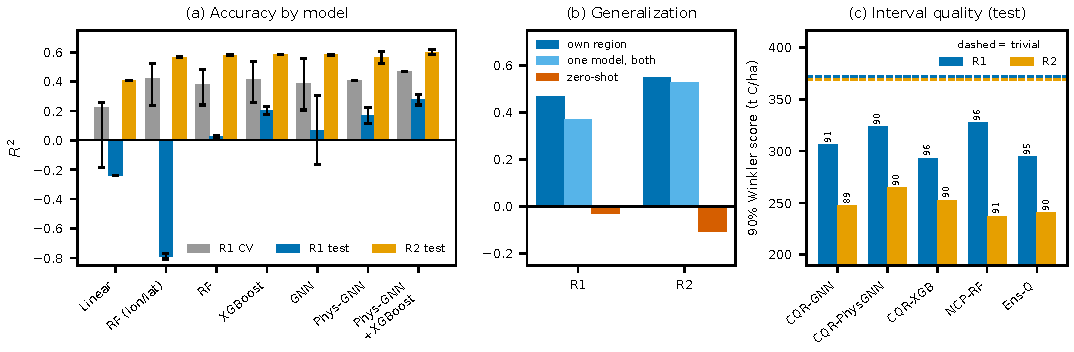
\includegraphics[width=0.97\linewidth]{figures/rev_fig1_results.pdf}
\caption{(a) $R^2$ by model: R1 cross-validation (whiskers: fold range) and test in R1 and R2 (mean $\pm$ SD, 3 seeds). (b) Ensemble generalization: own-region and two-region cross-validation, and zero-shot transfer (XGBoost, test). (c) 90\% Winkler score on test (lower is better); dashed lines: trivial interval; numbers: coverage (\%).}
\label{fig:results}
\end{figure*}

\subsection{Generalization and stability}
\DIFadd{A single ensemble trained on both regions reached cross-validated $R^2=0.37$ (R1) and 0.53 (R2)}\DIFaddend , \DIFdelbegin \DIFdel{pre-registered (Section~III-F)as the method to carry
forward, undercovered more at both levels, despite matching/exceeding
global there (Section~IV-B). One test node (of 2}%DIFDELCMD < {%%%
\DIFdel{,}%DIFDELCMD < }%%%
\DIFdel{076) got an inverted (empty)
interval under block-local correction at both levels, floored to zero
width and excluded from Section~VI's pricing examples; either way it
counted as a coverage miss. }\DIFdelend \DIFaddbegin \DIFadd{against 0.47 and 0.55 for region-specific models, whereas models applied to a region they had not seen scored below zero (}\DIFaddend Fig.~\ref{fig:results}(b)\DIFdelbegin \DIFdel{plots both
against the $y=x$ perfect-calibration line.
}%DIFDELCMD < 

%DIFDELCMD < \begin{figure*}[t]
%DIFDELCMD < \centering
%DIFDELCMD < 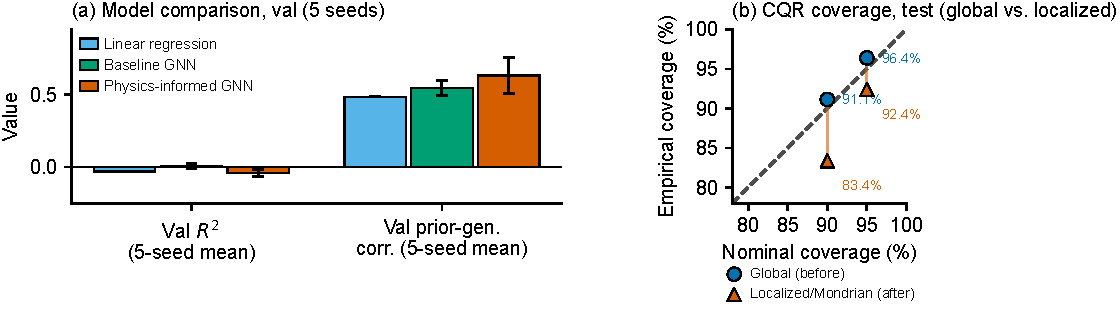
\includegraphics[width=0.95\linewidth]{figures/fig2_results.pdf}
%DIFDELCMD < \caption{(a) Validation $R^2$ and prior-gen.\ correlation, three models,
%DIFDELCMD < mean $\pm$ 1 std.\ across 5 seeds (linear regression: deterministic, no
%DIFDELCMD < error bar). (b) Empirical vs.\ nominal CQR coverage, test split, global
%DIFDELCMD < vs.\ localized (Mondrian); dashed line: perfect calibration.}
%DIFDELCMD < \label{fig:results}
%DIFDELCMD < \end{figure*}
%DIFDELCMD < 

%DIFDELCMD < \section{Discussion}
%DIFDELCMD < 

%DIFDELCMD < \textbf{The physics term's point-accuracy advantage did not replicate.}
%DIFDELCMD < %%%
\DIFdel{An earlier single-seed pilot found }\DIFdelend \DIFaddbegin \DIFadd{).
In that zero-shot setting, conformal intervals calibrated on the source region covered 76--89\% of target validation nodes; recalibrating them on half of the target's validation nodes restored 88--97\%.
Training }\DIFaddend the physics-informed \DIFdelbegin \DIFdel{loss
(Eq.

~\ref{eq:physloss}) improved test }\DIFdelend \DIFaddbegin \DIFadd{GNN on both image dates raised the rank agreement of its predictions across dates from 0.44 to 0.88 and its }\DIFaddend $R^2$ \DIFdelbegin \DIFdel{over a no-physics baseline.The multi-seed check (Section~IV-A)
already showed this was fragile (physics-informed mean validation $R^2$
across 5 seeds ($-0.040$) sat below the baseline's ($+0.005$) even before
the corrected split and pre-registered $\lambda$), and the final test
evaluation confirms it: the no-physics baseline GNNhas the best test
$R^2$ of the three.
This is the actual finding, not reconciled with the earlier result by reframing; a single seed on a single split was not
reliable here.
}\DIFdelend \DIFaddbegin \DIFadd{with August imagery from $-0.29$ to 0.35, for a 0.02 loss with February imagery.

}\DIFaddend 

\DIFdelbegin %DIFDELCMD < \textbf{What does hold up, at a smaller margin.} %%%
\DIFdel{The physics-informed
model's predictions correlate with the imposed mass-balance proxy more
strongly than either non-physics model on every evaluation in this paper, multi-seed validation (0.632 vs.\ 0.544/0.486)and the single test
evaluation (0.755 }\DIFdelend \DIFaddbegin \subsection{Intervals and crediting}
\DIFadd{Table~\ref{tab:uq} and Fig.~\ref{fig:results}(c) summarize the selected intervals (conformalized quantile GNN, global calibration).
In R1 the intervals matched the trivial interval's width but scored 18\% better on the Winkler score, and their width ranked absolute errors ($\rho=0.54$, 95\% confidence interval 0.51--0.58); in R2 they were 32\% narrower than the trivial interval (191 }\DIFaddend vs.\ \DIFdelbegin \DIFdel{0.682/0.686).
This requires the same precise
interpretation as before: the proxy correlated against is the exact
quantity the physics loss trained toward, so this is a
}\emph{\DIFdel{prior-generalization}} %DIFAUXCMD
\DIFdel{check (whether the constraint transfers to
held-out nodes), not independent physical validation , which this AOI's
single-date, flux-tower-free data cannot supply.
Whether this correlation
reflects genuine physical behavior, not just successful optimization
against its own training target, is this paper's most significant open
question. Resolving it would require flux-tower or repeated field-plot
carbon-flux measurements at this AOI, which do not currently exist, the clearest concrete next step for extending this work beyond a proxy-based
prior. What changed under the corrected protocol is the effect's size, not its direction: a real but modest margin on test (0.069}\DIFdelend \DIFaddbegin \DIFadd{282\,t\,C/ha).
Mondrian calibration covered 87.9\% in R1, where only six validation blocks were available.
Applied per node, the VM0033 rule withheld a median 12.7\% (R1) and 2.1\% (R2) of credits; across all five interval methods, credited stock stayed within 0.84}\DIFaddend --0\DIFdelbegin \DIFdel{.073) , not
the 0.6-point gap the
single-seed pilot reported. This is a direct product of the pre-registered
protocol working as intended.
}\DIFdelend \DIFaddbegin \DIFadd{.90 (R1) and 0.95--0.98 (R2) of the buffer-only amount.
Interval width did not track 2010--2020 mangrove loss (Spearman $-0.06$ in both regions).
Among the seven blue carbon projects with issued credits (6.62 million), the median buffer was 11.0\% and 73.5\% of credits had been retired \mbox{%DIFAUXCMD
\cite{vrod2026}}\hskip0pt%DIFAUXCMD
.

}\DIFaddend 

\DIFdelbegin %DIFDELCMD < \textbf{Localized calibration did not improve on global, and that is
%DIFDELCMD < itself informative.} %%%
\DIFdel{Section~III-F pre-registered localized (Mondrian)CQR from validation-internal evidence, before test was read.
On test it
undercovered more than global at both levels (83.4\% vs.\ 90\% nominal;
92.4\% vs.

\ 95\%, against global's 91.1\%/96.4\%), likely because only 6
spatial superblocks had enough validation nodes ($\geq 30$) for a stable
local correction. This matches theory: \mbox{%DIFAUXCMD
\cite{mao2024validmodelfree} }\hskip0pt%DIFAUXCMD
shows that local
conformal validity needs calibration points dense enough within each
local region, an }\emph{\DIFdel{infill asymptotic}} %DIFAUXCMD
\DIFdel{requirement this AOI's
validation split plausibly did not satisfy, a density limit, not
evidence against localization.
Nor is the pattern isolated to this paper:
applying Mondrian calibration to real-estate valuation, Hjort }\DIFdelend \DIFaddbegin \begin{table}[t]
\caption{Intervals (90\%, test) and crediting}
\centering
\begin{tabular}{lcc}
\toprule
 & R1 & R2 \\
\midrule
Coverage & 91.5\% & 89.1\% \\
Mean width / trivial (t\,C/ha) & 273 / 274 & 191 / 282 \\
Winkler score / trivial & 306 / 372 & 247 / 369 \\
$\rho$(width, abs.\ error) & 0.54 & 0.15 \\
Median VM0033 deduction per node & 12.7\% & 2.1\% \\
Project coverage, independent errors$^*$ & 18\% & 33\% \\
Project coverage, correlated errors$^*$ & 91\% & 100\% \\
\bottomrule
\multicolumn{3}{l}{\footnotesize $^*$Realized errors of 2.5\,km pseudo-projects, validation data.}
\end{tabular}
\label{tab:uq}
\end{table}

\DIFadd{When node uncertainties were aggregated to 2.5\,km pseudo-projects as VM0033 prescribes (root-sum-of-squares, independent errors), the stated project uncertainty covered the realized aggregate error in 18\% (R1, 11 projects) and 33\% (R2, 45 projects) of cases and implied no deduction.
Treating errors as fully correlated covered 91\% and 100\% and implied median deductions of 14.6\% and 3.1\%.

}

\subsection{Field soil cores}
\DIFadd{The 87 mangrove cores of the Coastal Carbon Library \mbox{%DIFAUXCMD
\cite{ccn2023library} }\hskip0pt%DIFAUXCMD
were converted to 0--100\,cm stocks, using a quadratic organic-matter conversion of the form in Craft }\DIFaddend et al.\ \DIFdelbegin \DIFdel{\mbox{%DIFAUXCMD
\cite{hjort2023spatialavm} }\hskip0pt%DIFAUXCMD
report "little to no improvement" over global
in one scenario, cautioning that an apparent gain can instead reflect a
non-conformity score failing to capture spatial trends.
Localization
gains in asset-pricing conformal calibration are setting-dependent, not
automatic. }%DIFDELCMD < \textbf{Business implication:} %%%
\DIFdel{global (simpler, the only
method meeting nominal coverage on test) is defensible for near-term
deployment; Section~VI's pricing PoC uses global intervals accordingly.
Both methods still produce test-set widths (318--383}\DIFdelend \DIFaddbegin \DIFadd{\mbox{%DIFAUXCMD
\cite{craft1991loi} }\hskip0pt%DIFAUXCMD
fitted on 679 regional samples ($R^2=0.91$), and matched to nodes within 300}\DIFaddend \,\DIFdelbegin \DIFdel{t/ha)several times the
label's std.
\ dev.\ (87.6}\DIFdelend \DIFaddbegin \DIFadd{m.
At the 25 sites, the median absolute error was 10.1\% for the ensemble, 11.6\% for the physics-informed GNN, 16.5\% for XGBoost, 14.1\% and 15.1\% for the Sanderman and Radabaugh maps, and 15.0\% for a constant.
The Sanderman map ranked sites best (Spearman 0.63; ensemble 0.29).
The two published maps were uncorrelated at node level ($-0.10$ in R1).
For the 13 cores sampled to at least 50}\DIFaddend \,\DIFdelbegin \DIFdel{t/ha), wide, not falsely confident}\DIFdelend \DIFaddbegin \DIFadd{cm, field-calibrated intervals covered 85--92\% under leave-one-study-out and implied VM0033 deductions of 22--29\%}\DIFaddend .

\DIFdelbegin %DIFDELCMD < \section{Pricing Proof-of-Concept}
%DIFDELCMD < %%%
\DIFdelend \DIFaddbegin \begin{figure}[t]
\centering
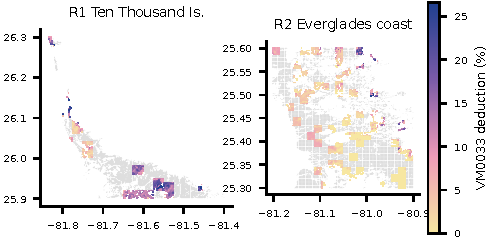
\includegraphics[width=0.98\linewidth]{figures/rev_fig2_deduction_map.pdf}
\caption{Per-node VM0033 uncertainty deduction (Eq.~\ref{eq:credit}) on test nodes of both regions, from 90\% conformal intervals. Gray: training and validation nodes.}
\label{fig:map}
\end{figure}

\DIFaddend 

\DIFdelbegin \DIFdel{CQR interval width measures present-day estimation confidence, }\DIFdelend \DIFaddbegin \section{Discussion}

\textbf{The physics-informed GNN and tree ensembles are complementary.} \DIFadd{Alone, the physics-informed GNN matched XGBoost in cross-validation (0.41 each), but their mean improved both regions (0.47 and 0.55) and held on test (0.28 and 0.60).
The GNN contributes neighborhood structure and the hydroperiod prior that the trees do not see, consistent with the control of tidal setting on mangrove soil carbon \mbox{%DIFAUXCMD
\cite{rovai2018controls}}\hskip0pt%DIFAUXCMD
, and it was also the most stable graph model across seeds and, once trained on both dates, across seasons.
The physics prior is now a weak constraint (correlation 0.14 with the predictions), }\DIFaddend not \DIFdelbegin \DIFdel{non-permanence risk (future carbon loss to erosion, disturbance,
sea-level rise) -- the quantity buffer pools price; this paper does not establish the two correlate. We illustrate, without validating, how }\DIFdelend \DIFaddbegin \DIFadd{a target the model copies.

}

\textbf{Estimation uncertainty is as large as the buffer the market already holds.} \DIFadd{The }\DIFaddend per-node \DIFdelbegin \DIFdel{estimation confidence could sit
alongside, not replace, a non-permanence buffer, built on }\emph{\DIFdel{global}}
%DIFAUXCMD
\DIFdel{CQR intervals per Section~V's recommendation, not }\DIFdelend \DIFaddbegin \DIFadd{deduction in R1 (12.7\%) is similar to the realized median buffer of issuing blue carbon projects (11.0\%), yet today it is not applied.
Fig.~\ref{fig:map} shows that the deduction concentrates in specific areas, so it is a location-dependent quantity that a flat buffer cannot represent.
Because width does not follow observed mangrove loss, }\DIFaddend the \DIFdelbegin \DIFdel{localized (Mondrian) variant it cautions against. A relative interval width is the 90\%-CQR
(global) width divided by the test set's own median (341.1\,t/ha; range
143.9--552.5\,t/ha). A price multiplier is
$1 - \alpha(\text{relative width}-1)$, clipped to $[0.5, 1.5]$, with
$\alpha=1.0$ an arbitrary illustrative sensitivity, not fit to market
outcome.
Table~\ref{tab:pricing} shows five nodes against Plan Vivo
V5.0's flat 20\% buffer .
}\DIFdelend \DIFaddbegin \DIFadd{two discounts measure different risks and belong in separate factors, as in Eq.~\ref{eq:credit}.
}\textbf{Business implication:} \DIFadd{a registry can adopt the deduction without changing its buffer policy.

}\DIFaddend 

\DIFdelbegin %DIFDELCMD < \begin{table}[htbp]
%DIFDELCMD < \caption{Pricing proof-of-concept: 5 representative test nodes (global CQR)}
%DIFDELCMD < \centering
%DIFDELCMD < \begin{tabular}{lccc}
%DIFDELCMD < \toprule
%DIFDELCMD < Node & Interval width & Our mult.\ & Flat-buffer mult.\ \\
%DIFDELCMD < \midrule
%DIFDELCMD < Min width  & 143.9 & 1.500 & 0.800 \\
%DIFDELCMD < p25        & 298.5 & 1.125 & 0.800 \\
%DIFDELCMD < Median     & 341.1 & 1.000 & 0.800 \\
%DIFDELCMD < p75        & 369.5 & 0.917 & 0.800 \\
%DIFDELCMD < Max width  & 552.5 & 0.500 & 0.800 \\
%DIFDELCMD < \bottomrule
%DIFDELCMD < \end{tabular}
%DIFDELCMD < \label{tab:pricing}
%DIFDELCMD < \end{table}
%DIFDELCMD < %%%
\DIFdelend \DIFaddbegin \textbf{Aggregation under independent errors is the weak point of the registry rule.} \DIFadd{Spatial model errors are correlated, so root-sum-of-squares aggregation shrinks project uncertainty and grants no deduction even where realized errors exceed the allowance.
A correlation-aware or empirically calibrated aggregation restored nominal coverage.
The same dependence explains why random validation overstates mapping accuracy \mbox{%DIFAUXCMD
\cite{ploton2020spatial} }\hskip0pt%DIFAUXCMD
and why Mondrian calibration undercovered with only six blocks \mbox{%DIFAUXCMD
\cite{mao2024validmodelfree}}\hskip0pt%DIFAUXCMD
.
Model-based crediting therefore needs an aggregation rule that accounts for spatial dependence.

}\DIFaddend 

\DIFdelbegin \DIFdel{Concretely, an issuer selling from both the well- (min-width) and poorly-characterized (max-width) node
above applies the identical 20\% discount today; under
a confidence-adjusted mechanism, the former prices at a 50\% premium,
the latter at a 50\% discount, a plausible implication, not a validated
outcome.

$\alpha$ and the clipping bounds are stated, arbitrary choices.
The flat-buffer value is not arbitrary: it is Plan Vivo V5.0's stated
buffer, used only as a comparison point (VM0033 instead scores a
project-specific value via its own risk tool, Section~I).
Fig.

~\ref{fig:spatial}
maps this interval width across the full test set, the spatial pattern
behind the location-differentiated pricing Table~\ref{tab:pricing}
illustrates.
}\DIFdelend \DIFaddbegin \textbf{What the intervals can and cannot do.} \DIFadd{Interval width is bounded by accuracy: with test $R^2=0.07$ for the GNN underlying the intervals in R1, at most about 4\% narrowing over the trivial interval is attainable, and in R2 ($R^2=0.58$) the 32\% achieved is close to the 35\% bound.
The value in R1 lies in adaptivity and Winkler score, not sharpness.
Local calibration is required when a model is moved to a new region, and at core scale even field-calibrated maps barely beat a regional mean, while at site scale the ensemble did.
Field-calibrated deductions (22--29\%) exceed label-calibrated ones, a reminder that the label product carries its own error, as fine-scale disagreement between soil carbon maps elsewhere has shown \mbox{%DIFAUXCMD
\cite{holmquist2018tidal}}\hskip0pt%DIFAUXCMD
.

}\DIFaddend 

\DIFdelbegin %DIFDELCMD < \begin{figure}[htbp]
%DIFDELCMD < \centering
%DIFDELCMD < 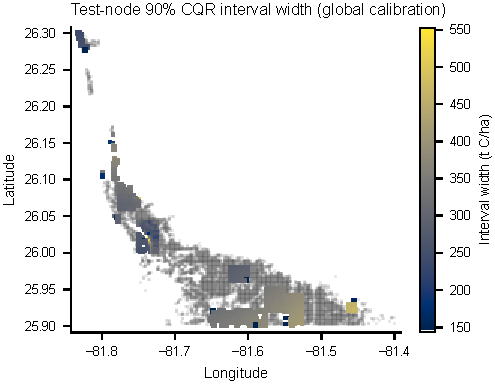
\includegraphics[width=0.95\linewidth]{figures/fig3_spatial_uncertainty.pdf}
%DIFDELCMD < \caption{Per-node 90\% global-CQR interval width, 2{,}076 test nodes
%DIFDELCMD < (\texttt{results/phase2\_cqr\_test\_predictions.csv}; range
%DIFDELCMD < 143.9--552.5\,t/ha, median 341.1\,t/ha, matching Table~\ref{tab:pricing}).
%DIFDELCMD < Gray: train/val nodes, for AOI context. Width clusters by location,
%DIFDELCMD < narrower northwest/centrally, wider south, the basis for
%DIFDELCMD < location-differentiated pricing.}
%DIFDELCMD < \label{fig:spatial}
%DIFDELCMD < \end{figure}
%DIFDELCMD < 

%DIFDELCMD < %%%
\DIFdelend \section{Limitations}
\DIFaddbegin \textbf{Labels are a modeled product:} \DIFadd{the training label is a global map that disagrees with a field-calibrated regional map at node level.
}\textbf{Accuracy in R1 is moderate} \DIFadd{($R^2=0.28$).
}\textbf{The ensemble was evaluated in a second test read,} \DIFadd{declared and limited to one pre-specified model.
}\textbf{Single tide gauges} \DIFadd{represent each region; R2's is about 70\,km away.
}\textbf{Field cores are sparse} \DIFadd{(13 deep enough for 0--100\,cm stocks) and may overlap the global map's training data.
}\textbf{Market outcomes} \DIFadd{were not modeled; prices and buffers come from published records.

}\DIFaddend 

\DIFdelbegin %DIFDELCMD < \textbf{Single-date imagery} %%%
\DIFdel{constrains the physics term to a
cross-sectional relationship, not an actual $dC/dt$ (not invalidating
the prior-generalization result, defined relative to that same proxy).
}%DIFDELCMD < \textbf{No flux/decomposition data} %%%
\DIFdel{exists for this AOI; accretion/export
are proxies (Section~III-E). }%DIFDELCMD < \textbf{Distance-to-gauge is a positional
%DIFDELCMD < proxy}%%%
\DIFdel{, not a tidal-energy layer.
}%DIFDELCMD < \textbf{The prior-generalization result
%DIFDELCMD < is not independent validation} %%%
\DIFdel{(Sections~III-F, V): it measures transfer, not physical correctness.
}%DIFDELCMD < \textbf{CQR excluded the physics loss}%%%
\DIFdel{, a
disclosed scope choice. }%DIFDELCMD < \textbf{Localized (Mondrian) CQR undercovered on
%DIFDELCMD < test} %%%
\DIFdel{(Section~IV-C, V) , a data-density limit here, not spatial
calibration generally \mbox{%DIFAUXCMD
\cite{lou2024geoconformal,mao2024validmodelfree}}\hskip0pt%DIFAUXCMD
.

}%DIFDELCMD < \textbf{Single region}%%%
\DIFdel{; the five-seed check addresses seed variance, not
regional generalization.
}%DIFDELCMD < \textbf{The pricing mechanism is illustrative}%%%
\DIFdel{,
with an unfit sensitivity parameter and no market validation.
}%DIFDELCMD < \textbf{The graph has 2{,}520 directed edges (3.92\%) crossing split
%DIFDELCMD < boundaries} %%%
\DIFdel{(9.7\% of nodes, 14.2\% of test nodes, are 1-hop neighbors
across a split); restricting Table~\ref{tab:threeway} to the 1}%DIFDELCMD < {%%%
\DIFdel{,}%DIFDELCMD < }%%%
\DIFdel{782
non-boundary test nodes gives lower $R^2$ for all three models (linear
$-0.504$, baseline GNN $-0.447$, physics GNN $-0.494$) but the same
ranking, so reported numbers carry a small, non-model-specific optimistic
bias from this leakage.

}%DIFDELCMD < \textbf{The single test-side seed, the untested random-forest baseline,
%DIFDELCMD < and the pricing mechanism's gaming-risk and registry-adoption questions}
%DIFDELCMD < %%%
\DIFdel{remain unaddressed.
}%DIFDELCMD < 

%DIFDELCMD < %%%
\DIFdelend \section{Conclusion}
\DIFdelbegin %DIFDELCMD < 

%DIFDELCMD < %%%
\DIFdel{A pre-registered, two-stage protocol (validation-only selection, single
held-out test confirmation) caught two overstated results a single run
would have missed: an earlier single-seed pilot's headline finding, and a
theoretically-motivated localized calibration refinement favorable on
validation-internal evidence alone. What survives (the }\DIFdelend \DIFaddbegin \DIFadd{Calibrated per-node uncertainty from a }\DIFaddend physics-informed \DIFdelbegin \DIFdel{model's smaller but real prior-generalization advantage, }\DIFdelend \DIFaddbegin \DIFadd{GNN and XGBoost ensemble can supply the VM0033 uncertainty deduction.
Across two regions and two image dates, the ensemble reached test $R^2=0.28$ and 0.60, intervals reached 89--92\% coverage, and the deduction (median 12.7\% in R1) is comparable to the 11.0\% buffers that issuing projects hold.
The methodology's independent-error aggregation covered only 18--33\% of realized project errors, and against 87 field cores the ensemble's site-level error (10.1\%) was below both published maps and a regional mean.
Future work will test a correlation-aware aggregation with registry project data, add regions with denser field cores, }\DIFaddend and \DIFdelbegin \DIFdel{honestly
wide, node-differentiated CQR intervals ) are two separate results, not
one flowing from the other: the CQR pipeline priced here used data loss
only , without the physics term.
Together they motivate the market-facing
contribution: an estimation-confidence signal that could complement, not
replace, flat buffer pools, deployed here on the simpler,
better-calibrated global variant. Future work : a second
Sentinel-2 date, a higher-volume or second-region localized-conformal
test, deep-ensemble/MC-dropout comparisons, and market-outcome validation
of the pricing mechanism against non-permanence risk}\DIFdelend \DIFaddbegin \DIFadd{replace the steady-state prior with repeated elevation and accretion measurements.

}

\section*{\DIFadd{Code Availability}}
\DIFadd{Code, data pipeline, selection rules and results: }\url{https://github.com/Nahla-Nabil/PIGNN-UQ}\DIFaddend .

\bibliographystyle{IEEEtran}
\bibliography{references}

\end{document}
